% !TEX root = BA-Bauer
\newpage
\section{Software}
In diesem Kapitel werden die Funktionsweisen der wichtigsten Funktionen der Software erläutert, sowie die Hilfsmittel die zur Erstellung des Programmcodes verwendet werden, vorgestellt. Der vollständige Programmcode, sowie Projektdateien befinden sich im Anhang \ref{CD-Anhang}, sowie als git-repository \cite{git_bpa_code} und \cite{git_lcd} auf github.com.
% !TEX root = BA-Bauer.tex
\subsection{Hardwareabstraktionsschicht HAL (Hardware Abstraction Layer)}
Bei der Programmierung eines Mikrocontrollers muss selbstverständlich eine für den Mikrocontroller verständliche Sprache gesprochen werden. Möchte man beispielsweise ein Byte mithilfe der UART-Schnittstelle senden, so muss der intern verbundene entsprechnende Pin das Signal ausgeben. Wird nun der selbe Programmcode für einen anderen Mikrokontroller verwendet, ist der Ausgangspin des UARTs eventuell ein anderer und der Programmcode wird nicht funktionieren. Die Lösung des Problems ist entweder das Ändern des Programmcodes oder die Verwendung der Hardwareabstraktionsschicht (HAL). Die HAL trennt die Anwendungsschicht von der Hardwareschicht, sodass der Programmcode unabhängig von der Hardware geschrieben werden kann. Bei der Programmierung werden HAL-Funktionen aufgerufen, welche dann die entsprechenden Hardware-Operationen durchführen. Die HAL ist außerdem in einzelne Komponenten aufgeteilt, wie z.B. die UART-Schnittstelle oder Timer \cite[S.77 ff.]{IoTSystems}. Als Beispiel soll ein Byte über die UART-Schnittstelle gesendet werden. Im Hauptprogramm wird dafür die Funktion $HAL\_UART\_Transmit(...)$ aus der Datei $stm32f4xx\_hal\_uart.c$ aufgerufen. In dieser Funktion wird die UART-Schnittstelle für das Senden vorbereitet, das Byte in das entsprechende Datenregister geschrieben und anschließend der Sendevorgang gestartet. Dabei werden in der Funktion nur bestehende Konstanten der Registeradressen verwendet. Diese Konstanten sind in der Datei $stm32f446xx.h$ definiert. Soll der Programmcode nun auf einem STM32F401CE Mikrocontroller laufen, so muss lediglich die Datei $stm32f446xx.h$ ersetzt werden. Voraussetzung dafür ist, dass alle Schnittstellen, die im Programmcode verwendet werden, auch in dem neuen Mikrocontroller existieren. Die HAL-Treiber und Definitionen der Mikrocontroller müssen in der Regel nicht händisch programmiert werden, sondern werden vom Hersteller des Mikrocontrollers zur Verfügung gestellt. STMicroelectronics bietet darüber hinaus kostenlose Software mit der der Umgang mit den hochkomplexen Mikrocontrollern vereinfacht wird.
%!TEX root = BA-Bauer.tex

\subsection{STMicroelectronics CubeMX}
Die Firma STMicroelectronics\textsuperscript{®} bietet für Programmierung der eigenen Mikokontrollern und -porzessoren eine Reihe von kostenloser Software zum Download an. Darunter befindet sich unter anderem die Software CubeMX, die für jeden Mikrocontroller und jedes Entwicklungsboard von STMicroelecronics\textsuperscript{®} verwendet werden kann. Mit der Software können Schnittstellen, Ein und Ausgangspins, Einstellungen der Taktgebung und vieles mehr in einer grafischen Benutzeroberfläche vor der eigentlichen Programmierung konfiguriert werden, was das Durchsuchen des Handbuchs nach den entsprechenden Registern überflüssig macht. CubeMX generiert .c und .h Dateien mit diversen Funktionen für die konfigurierten Schnittstellen und der Hardware. 

Abbildung \ref{fig:CubeMXClock} zeigt die Benutzeroberfläche zur Konfiguration der Taktgebung in CubeMX. 
\begin{figure}[h]
	\centering
	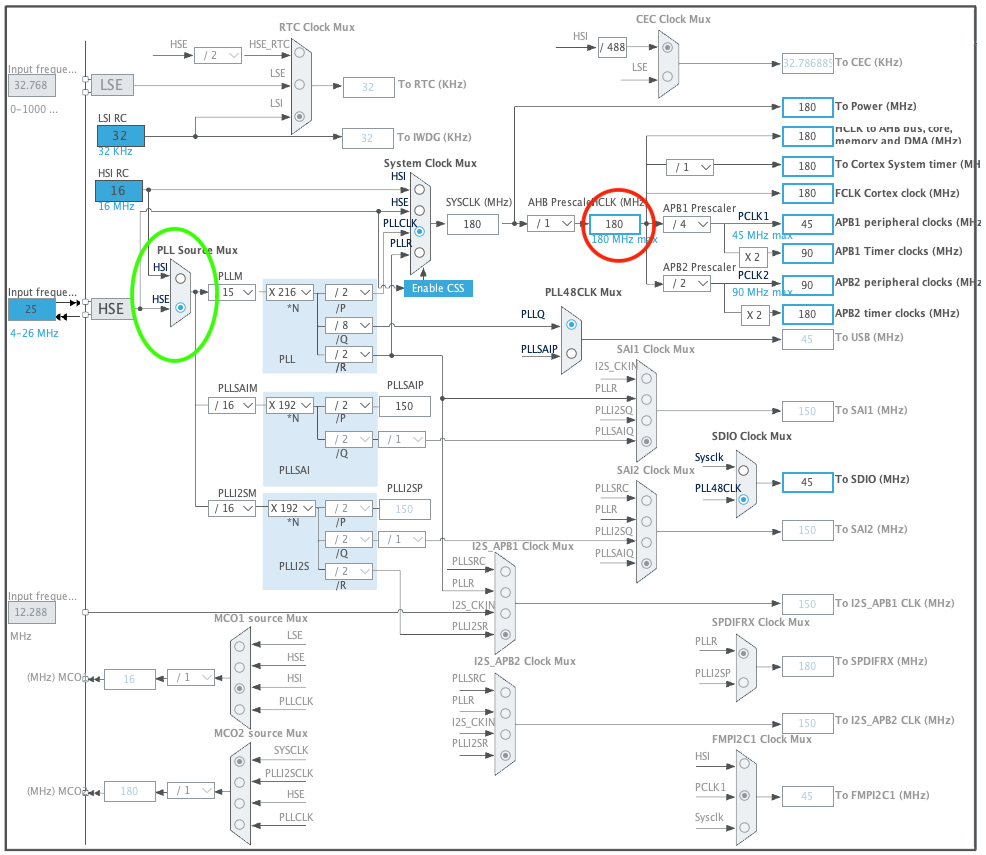
\includegraphics[width=.5\linewidth]{CubeMX-clock-mark}
	\caption{CubeMX Clock Configuration}
	\label{fig:CubeMXClock}
\end{figure}
Die Oberfläche ist nach der Flussrichtung der Taktsignale durch die Parameter und Umschalter angeordnet. Auf der linken Seite finden sich die Oszillatoren, dessen Frequenz durch die in der Mitte befindlichen Parameter und Umschalter geteilt oder multipliziert werden kann. Auf der rechten Seite befinden sich die ausgehenden Taktfrequenzen für die einzelnen Schnittstellen. Um den externen Hochfrequenzoszillator zu verwenden, wird im grün markierten Bereich der $HSE$ Umschalter aktiviert und die Frequenz des Oszillators links neben dem grün markierten Bereich einegeben. Damit der Mikrocontroller mit der maximalen Taktfrequen von 180\,MHz arbeitet wird das rot markierte Feld mit 180 beschrieben. CubeMX berechnet alle Parameter und Umschalter um die gewählte Taktfrequenz des Mikrocontrollers und der verwendeten Schnittstellen zu erreichen. Anhand der großen Anzahl an Variablen ist das Einstellen der Parameter und Umschalter per Hand nur mit sehr großem Aufwand zu bewerkstelligen. CubeMX unterstützt den Prozess des Programmierens auch in der Konfiguration von Schnittstellen. Der in dieser Arbeit verwendete STM32F446ZE Mikrokontroller besitzt 20 Schnittstellen welche ohne CubeMX einzeln durch das Beschreiben von Registern konfiguriert werden müssten. Mit CubeMX können diese Schnittstellen mithilfe einer grafischen Oberfläche eingestellt werden. Zudem schlägt die Software verwendbare Pins zu den jeweiligen Schnittstellen vor, welche durch die Zuweisung an einem virtuellen Mikrocontroller der Schnittstelle zugeordnet werden kann. Die Pins des Mikrocontrollers besitzen unter Umständen mehrere Funktionen gleichzeitig, können jedoch nur von einer Schnittstelle parallel verwendet werden.  Solche Überschneidungen werden von CubeMX erkannt und können manuell durch die Zuweisung eines anderen noch verfügbaren Pins behoben werden. 
%\begin{figure}[h] 
%	\centering
%	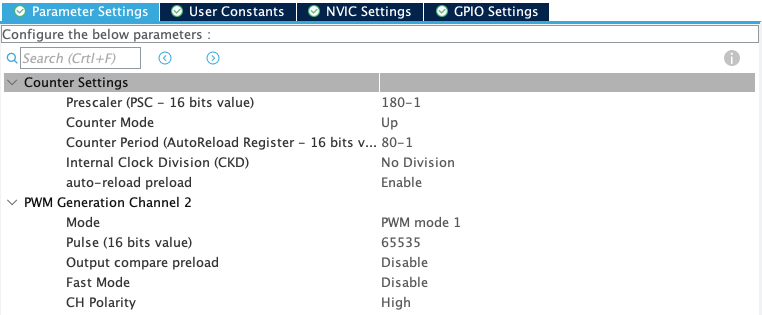
\includegraphics[width=.5\linewidth]{CubeMX-timerconfig}
%	\caption{CubeMX Beispiel Schnittstellenkonfiguration Timer}
%	\label{fig:CubeMXTimer}
%\end{figure}
%Schnittstellenzuweisung der Pins
%Funktionen der Pins
%Interrupts etc. aktivieren
%Koniguration der Schnittstellen
%HAL?!?!
% !TEX root = BA-Bauer.tex

\subsection{STMicroelectronics STM32CubeIDE}
Nachdem der Grundcode von CubeMX generiet ist, wird der Programmcode mithilfe der Entwicklungsumgebung STM32CubeIDE von STMicroelectronics erstellt. Sie ist speziell für die Entwicklung von Programmcode für STM32 Mikcontroller und -prozessoren ausgelegt und beinhaltet neben der Kompilierung von Code auch debugging-Funktionalität. Durch die Einbindung von CubeMX in der Entwicklungsumgebung wird keine weitere Software zum porgrammieren eines STM32 Mikrocontrollers oder -prozessors benötigt. Jederzeit kann die Kofiguration in CubeMX geändert und ein neuer Grundcode generiert werden \cite{CubeIDE}. Code der vom Benutzer geschrieben wurde, wird bei diesem Vorgang nicht verändert. Voraussetzung dafür ist die richtige Position des Benutzer-Programmcodes innerhalb der $USER\ CODE$-Blöcke (\ref{code:usercode}).
\lstinputlisting[
caption = main.c: USER CODE Block,
label = code:usercode, 
language = C, 
firstnumber = 106, 
firstline = 106, 
lastline = 108]
{/Users/Felix/Documents/CubeMX/BPA-Code/Core/Src/main.c}
Code der zwischen der $BEGIN$ und $END$-Zeile geschrieben steht, wird bei einer Neugenerierung beibehalten. Diese Blöcke finden sich an verschiedenen Stellen und Dateien wieder.
% !TEX root=BA-Bauer.tex

\subsection{Taster}
Um eine einwandfreie Funktion der Taster zu garantieren ist nicht nur deren Schaltung, sondern auch ein entsprechender Programmcode wichtig. Im folgenden Kapitel wird auf den Programmcode, der zum auslesen eines Tasterdrucks verwendet wird, eingegangen. Ein Tasterdruck kann zu jedem Zeitpunkt des Programmablaufs geschehen und sollte möglichst vom Porgrammcode nicht unbeachtet bleiben. Um diese Funktionalität zu gewährleisten, sind die Taster mit interruptfähigen Eingängen des MCUs verbunden. Die Beschaltung des Tasters mit einem im MCU internen Pull-Up-Widerstand sorgt dafür, dass an den Tastern im nicht betätigten Zustand ein High-Pegel und während der Betätigung ein Low-Pegel anliegt. Der Interrupt muss also auslösen, wenn sich der Logikpegel eines Tasters von einem High- auf einen Low-Pegel ändert, also eine fallende Flanke des Taster-Signals erkannt wird. In CubeMX werden die Taster-Pins so konfiguriert, dass eine Interrupt-Routine beim Auftreten einer fallenden Flanke aufgerufen wird. Diese Routine ruft eine sogenannte Callback-Funktion auf, in der die Betätigung des Tasters bearbeitet wird. Code-Ausschnitt \ref{code:btn.h} zeigt einen Ausschnit aus der Datei button.h. Jedem Taster wird ein Zahlenwert der Basis 2 zugewiesen. Diese Spiegeln die Bits 1-4 eines Bytes wieder.
\lstinputlisting[
caption = button.h: Definitionen und Funktionsprototypen,
label = code:btn.h, 
language = C, 
firstnumber = 5, 
firstline = 5, 
lastline = 12]
{/Users/Felix/Documents/CubeMX/BPA-Code/Core/Inc/button.h} 
Codeausschnitt \ref{code:btn.c} zeigt einen Teil der Callback-Funktion. Zunächst wird in Zeile 30 geprüft ob in den letzten 200\,ms ($DELAYTIME$) bereits ein Aufruf der Funktion erfolgt ist. Diese Abfrage soll mehrfache Eingaben, augelöst durch ein mechanisches Schwingen des Tasters verhindern. Falls sie bereits aufgerufen wurde, so wird die Funktion beendet, da der Aufruf wahrscheinlich durch das mechanische Schwingen des Taster aufgerufen wurde. Falls nicht wird die Variable $last\_updated$ mit der aktuellen Zeit aktualisiert. Daraufhin wird mithilfe einer $switch$-Anweisung festgestellt welcher Taster den Interrupt ausgelöst hat. Dafür wird die Variable $GPIO-Pin$, welche von der Interrupt-Funktion an die Callback-Funktion übergeben wird, mit den einzelnen Pins der Taster verglichen. 
\lstinputlisting[
caption = button.c: Codeausschnitt Taster-Interruptfunktion,
label = code:btn.c, 
language = C, 
firstnumber = 28, 
firstline = 28, 
lastline = 33]
{/Users/Felix/Documents/CubeMX/BPA-Code/Core/Src/button.c}
Ist der auslösende Pin festgestellt, wird der Variable $presses$ mithilfe einer bitweisen $oder$-Operation der entsprechende Zahlenwert des Tasters, der in der Datei $button.h$ (Codeausschnitt \ref{code:btn.h} definiert ist, wie folgt zugewiesen.
\lstinputlisting[
caption = button.c: Bitweise Zuordnung eines betätigten Tasters,
label = code:bitwise_or, 
language = C, 
firstnumber = 37, 
firstline = 37, 
lastline = 41]
{/Users/Felix/Documents/CubeMX/BPA-Code/Core/Src/button.c}
Der Vorteil der bitweisen $oder$-Operation ist, dass nur das entsprechende Bit gesetzt wird ohne alle anderen zu verändern. Ergänzende Abfragen ob das Bit bereits gesetzt ist entfallen.
Im Hauptprogramm werden ausschließlich die Funktionen $Button\_pressed(uint8\_t)\ button)$ für die Abfrage ob ein bestimmter Taster betätigt wurde und $Button\_reset()$ um die Variable $presses$ zurückzusetzen verwendet. Bei der Abfrage eines Tasters wird das entsprechende Bit wieder zurückgesetzt. Wurden zwei verschiedene Taster innerhalb kurzer Zeit betätigt, können beide nacheinander oder gleichzeitig mit der Funktion $Button\_pressed(...)$ abgefragt werden. Codeausschnit \ref{code:btn_pressed} zeigt den Inhalt dieser Funktion. Zunächst folgt eine $if$-Abfrage wann die letzte Tastereingabe registriert wurde. Ist die Eingäbe nicht älter als der Wert von $TIMEOUT$, so wird zunächst die temporäre Variable $temp$ mit dem Wert 0 beschrieben. Mithilfe einer bitweisen $und$-Operation der durch die Callback-Funktion beschriebenen Variable $presses$ und dem Wert des abgefragten Tasters wird die Variable $temp$ mit dem entsprechenden Wert beschrieben. Zuletzt werden die abgefragten Bits aus der Variable $presses$ mit einer $0$ überschrieben. Der Rückgabewert der Funktion ist die Variable $temp$. Im Hauptprogramm kann anhand eines Rückgabewertes ungleich $0$ erkannt werden, dass der oder einer der abgefragten Taster betätigt wurde.
\lstinputlisting[
caption = button.c: Abfrage eines Tasters,
label = code:btn_pressed, 
language = C, 
firstnumber = 10, 
firstline = 10, 
lastline = 21]
{/Users/Felix/Documents/CubeMX/BPA-Code/Core/Src/button.c}
Zur Veranschaulichung des Ablaufs der Funktion soll im Folgenden als Beispiel abgefragt werden, ob der Zurück-Taster betätigt wurde. Im Hauptprogramm wird die Funktion \textit{Button\_pressed(BACK)} dazu aufgerufen. Die Konstante $BACK$ besitzt den Wert 1, also Binär 0000 0001. Kurz bevor die Funktion aufgerufen wurde, wurde der Zurück- und Bestätigung-Taster betätigt. Der Inhalt der Variable $presses$ ist dadurch Binär 0000 0011. Die bitweise $und$-Operation der beiden Variablen ergibt Binär 0000 0001. Der Rückgabewert der Funktion ist somit 1 und damit kann im Hauptprogramm von einer Betätigung des Zurück-Taster ausgegangen werden. Wird nun allerdings die gleiche Funktion ein zweites Mal aufgerufen, ohne das der Zurück-Taster betätigt wurde, so ist der Inhalt der Variable $presses$ Binär 0000 0010. Das Bit des Zurück-Taster wurde mithilfe der Operation in Zeile 19 zurückgesetzt. Die $und$-Operation hat dann das Ergebnis 0000 0000. Der Rückgabewert der Funktion ist null, der abgefragte Taster ist nicht betätigt worden.
\newline
\textbf{Optimierungsmöglichkeiten}\\
Die Konstante $TIMEOUT$ besitzt keine Zuordnung zu einem einzelnen Taster. Wurde vor längerer Zeit ein Taster betätigt und kurz vor der Abfrage ein anderer Taster betätigt, so scheint die Betätigung des ersten Tasters auch innerhab der Timeout-Zeit geschehen zu sein. Dieses Problem kann gelöst werden, indem eine Variable pro Taster angelegt wird, in der die Zeit der letzten Betätigung des jeweiligen Tasters gespeichert wird. Diese ersetzt die globale letzte Aktualisierungszeit $last\_updated$. Der Nachteil dieser Methode ist eine deutlich aufwendigere Abfrage in der Funktion $Button\_pressed(...)$ und Zuweisung in der Callback-Funktion. Eine zweite Möglichkeit das Problem zu lösen ist der Einsatz eines Timers. Dieser wird gestartet wenn ein Taster betätigt wird. Läuft der Timer über, wird in der Interrupt-Funktion des Timers der Betätigungszustand in der Variable $presses$ für alle Taster zurückgesetzt. Soll nur der Zustand eines Tasters zurückgesetzt werden, so muss je ein Timer pro Taster zur Verfügung stehen, da in der Interupt-Funktion des Timers nicht unterschieden werden kann welcher Taster den Timer gestartet hat.
% !TEX root = BA-Bauer.tex

\subsection{Encoder}
Für den Programcode des Encoders kommt ein ähnliches Prinzip wie für die Taster im vorherigen Kapitel zum Einsatz. Der Aufruf der entsprechenden Funktion erfolgt über einen Interrupt.
Wie bereits in Kapitel \ref{sec:Encoder} beschrieben, muss der Zustand beider Terminals des Encoders ausgelesen werden um eine Drehrichtung bestimmen zu können. Terminal $A$ ist in CubeMX als externer Interrupteingang mit Erkennung einer fallenden Flanke, Terminal $B$ als Standard-Eingang konfiguriert. Wird durch eine fallende Flanke des Signals des Terminals $A$ ein Interrupt ausgelöst, so entscheidet der Zustand des Terminals $B$ über die Drehrichtung des Encoders. In der Interrupt-Funktion muss also lediglich der Zustand von Terminal $B$ geprüft werden. 
\lstinputlisting[
caption = Encoder.c: Interrupt-Funktion,
label = code:enc.c, 
language = C, 
firstnumber = 45, 
firstline = 45, 
lastline = 60]
{/Users/Felix/Documents/CubeMX/BPA-Code/Core/Src/Encoder.c}
Codeausschnitt \ref{code:enc.c} zeigt den Inhalt der Interruptfunktion. Zunächst wird in Zeile 47-49, wie auch in der Interrupt-Funktion der Taster, eine softwareseitige Entprellug durchgeführt. Die Verzögerungszeit fällt für den Encoder mit 50\,ms deutlich kürzer aus als für die Taster, um auch schnelle Drehbewegungen registrieren zu können. Eine längere Verzögerungszeit hat einen Verlust von getätigten Eingaben, besonders bei höheren Drehgeschwindigkeiten, zur Folge. 50\,ms haben sich in Tests als angenehm zu bedienen erwiesen und einen guten Kompromiss zwischen maximaler Eingabegeschwindigkeit und Zuverlässigkeit der Eingaben hergestellt.
Nach der Entprellung folgt die Abfrage des Zustands des Terminals $B$ mithilfe der Funktion $HAL\_GPIO\_ReadPin(...)$. Ist der Zustand $High$, so wird die global verfügbare Variable $enc\_position$ um 1 dekrementiert, wenn sie größer als 0 ist. Ist der Zustand $Low$, so wird die Variable um 1 inkrementiert. Bei der Variable $enc\_position$ handelt es sich um eine 16-Bit Variable ohne Vorzeichen, welche $2^{16} = 65536$ Werte umfasst und damit genug Platz für Eingaben bietet.\\
\newline
\textbf{Optimierungsmöglichkeiten}\\
Bei der Entwicklung des Schaltplans ist ein Fehler im Bereich der CR-Filter zum Entprellen des Encoders nach der Fertigung der Platine aufgefallen. Durch diesen Fehler wird die Filter-Beschaltung des Encoders unwirksam im Bezug auf dessen Entprellung. Mit der Behebung könnte die softwareseitige Entprellung reduziert werden oder sogar vollständig entfallen. Dadurch kann die Responsivität des Encoders verbessert werden.
Außerdem wäre eine Erkennung der Drehgeschwindigkeit sinnvoll um bei einer größeren Geschwindigkeit die Inkrement- und Dekrementgröße zu variieren, wodurch schnellere und präzise Eingaben gleichermaßen möglich sind.
% !TEX root = BA-Bauer.tex

\subsection{DMX-Struktur}
\label{sec:dmx_struct}
Informationen die für die Aufnahme oder Wiedergabe der DMX-Daten benötigt werden, werden an verschiedenen Stellen des Programms eingeholt und an anderen Stellen wiederrum benötigt. Um die Informationen einfach zugänglich zu machen, werden diese mithilfe einer Struktur gebündelt. Abbildung \ref{code:dmx-struct} zeigt die Definition dieser Struktur, welche von der Praxisprojektarbeit übernommen und erweitert ist. Die Struktur ähnelt einer Klassendefinition in C++. Durch die Deklaration einer Instanz der Struktur zum Beispiel mit dem Namen $Univers$, können die Variablen der Struktur über die Instanz erreicht werden. Die Variable $rec_time$ würde über $Univers.rec_time$ erreichbar sein und kann gelesen und beschrieben werden. Damit die Instanz an allen Stellen im Programm verwendet werden kann, wird sie global definiert. Die in den folgenden Kapitel verwendeten Variablen werden den in dieser Struktur befindlichen zugewiesen oder die Werte aus ihnen gelesen.
\lstinputlisting[
caption = DMX.h: Typdefinition DMX\_TypeDef,
label = code:dmx-struct, 
language = C, 
firstnumber = 24, 
firstline = 24, 
lastline = 39]
{/Users/Felix/Documents/CubeMX/BPA-Code/Core/Inc/DMX.h}
% !TEX root = BA-Bauer.tex

\subsection{Aufnahmefunktionen}
\label{sec:recfunctions}
Für die Aufnahme von DMX-Daten stehen insgesamt vier verschiedene Aufnahmemodi zur Verfügung, welche jeweils eine Aufnahmefunktion bilden. Der erste Aufnahmemodus ist der Standard-Modus, bei dem vorab die Dauer der Aufnahme festgelegt wird. Nach Ablauf der Aufnahmedauer stoppt die Aufnahme und kehrt zum Menü zurück. Der zweite Modus ist der sogenannte $Trigger$-Modus, bei dem zuvor in den Einstellungen ein $Trigger$-Kanal und $Trigger$-Wert festgelegt wird. Ist die Aufnahme gestartet und in den eingehenden DMX-Datenpaketen wird der $Trigger$-Wert des ausgewhählten $Trigger$-Kanals überschritten, so startet ab diesem Zeitpunkt die Speicherung der DMX-Daten. Die Aufnahme wird gestoppt, wenn der $Trigger$-Wert wieder unterschritten wird. Dieser Modus ermöglich das Starten und Stoppen der Aufnahme zu sehr präzisen Zeitpunkten. Vor allem für sich wiederholende Bewegungsabläufe von Lichttechnischen Geräten ist diese Funktion äüßerst sinnvoll. Ist die Position eines Lichtkegels beispielsweise am Anfang und Ende der Aufnahme identisch, so kann die Aufnahme endlos nacheinander wiedergegeben werden, ohne dass ein Anfang oder Ende der aufgenommenen Sequenz sichtbar ist. Der letzte kontinuierliche Aufnahme-Typ ist die endlose Aufnahme, bei der die Aufnahme ohne die Wahl einer Aufnahmedauer gestartet wird und durch betätigen des Zurück-Tasters gestoppt wird. Dieser Modus richtet sich an Situationen, in denen die Endzeit der Aufnahme beim Aufnahmebeginn nicht festgelegt werden kann. Ein Beispiel für einen Anwendungsfall ist ein Konzert. Zu beginn des Konzerts kann die Aufnahme gestartet werden und nachdem die letzte Zugabe gespielt ist, wieder gestoppt werden. Bei dem letzten Aufnahme-Typ handelt es sich um eine nicht-kontinuierliche Aufnahme der DMX-Daten, die sogenannte $Step$-Aufnahme. Bei diesem Aufnahme-Typ können einzelne Datenpakete des eingehenden DMX-Datenstroms aufgenommen werden. Jedes Datenpaket entspricht einem $Step$ und enthält, im Gegensatz zu den drei anderen Aufnahmemodi, keine Zeitinformationen. Die einzelnen Steps werden bei der Wiedergabe in einem regelmäßigen Zeitabstand, der erst bei der Wiedergabe vom Benutzer festgelegt wird, wiedergegeben. Dieser Modus gibt dem Benutzer die Möglichkeit die DMX-Datenpakete in einer bestimmten Taktung auszugeben und diese beispielweise an den Takt eines Liedes anzupassen. Zudem wird durch die Speicherung einzelner Datenpakete, im Vergleich zu den anderen Aufnahmemodi, deutlich weniger Speicherplatz auf der SD-Karte benötigt. 
Im Folgenden wird auf das Grundprinzip der Aufnahmefunktionen eingegangen. Ein Flussdiagramm des Standard-Aufnahmemodus befindet sich im Anhang \ref{fluss:recf}.\newline
Die drei Aufnahmemodi der kontinuierlichen Aufnahme, also Standard-, Endlose- und $Trigger$-Aufnahme unterscheiden sich im wesentlichen nur in den Start- bzw. Stoppbedingungen. Im Standardmodus muss zusätzlich eine Aufnahmezeit festgelegt werden. 
\begin{table}[h]
	\begin{center}
		\begin{tabular}{l | p{6cm} | p{6cm}}
			Modus & Startbedingung & Stoppbedingung\\
			\hline
			Standard & Bestätigungstaster & Ablauf der Aufnahmezeit\\
			Endlos & Bestätigungstaster & Zurück-Taster\\
			$Trigger$ & $Trigger$-Wert auf $Trigger$-Kanal überschreiten & $Trigger$-Wert auf $Trigger$-Kanal unterschreiten
		\end{tabular}
	\end{center}
\end{table}\newline
\subsubsection{Festlegen der Aufnahmezeit}
Abbildung \ref{lcd:rectime} zeigt die Ausgabe auf dem LCD-Display für die Festlegung der Aufnahmezeit. Die Auswahl der Zeit ist in vier Blöcke für das Einstellen der Stunden, Minuten, Sekunden und Millisekunden aufgeteilt. Mit den Links- und Rechts-Tastern kann der ausgewählte Block, markiert mit dem Zeichen in der untersten Zeile des Displays, verändert werden. 
\begin{figure}[h]
	\begin{center}
		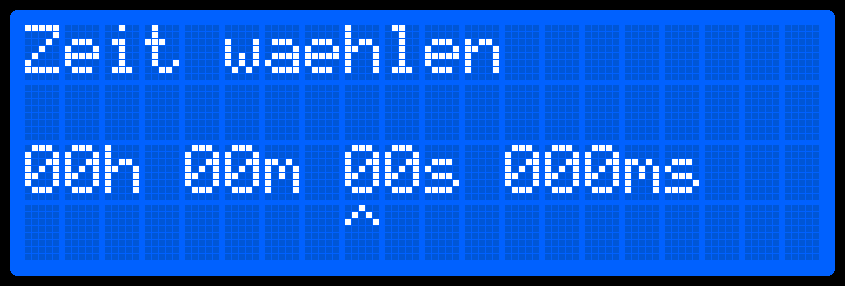
\includegraphics[width=.25\linewidth]{LCD-Screenshots/Zeitauswahl}
		\caption{LCD-Ausgabe Aufnahmezeit}
		\label{lcd:rectime}
	\end{center}
\end{figure}
Der Wert des Blocks wird mit einer Drehung des Encoders im Uhrzeigersinn erhöht und gegen den Uhrzeigersinn verringert. Der Millisekunden-Block erhöht, bzw. verringert sich immer um 10 Millisekunden. Eine feinere Auflösung im Millisekundenbereich ist nicht sinnvoll, da die DMX-Datenpakete eine Zeitdauer von 22\,ms zur vollständigen Übertragung benötigen. Wird eine Drehbewegung des Encoders registriert, so wird zunächst überprüft ob der vorherige Wert weiter erhöht oder verringert werden kann. Damit wird ausgeschlossen, dass eine Zeit kleiner null gewählt werden kann oder beispielsweise die Anzahl der Minuten größer 59 ist. Ist die Auswahl der Zeit beendet so muss sie mit dem Bestätigung-Taster bestätigt werden. Die eingegebene Zeit wird dann in Millisekunden umgerechnet und in die entsprechende Variable der Aufnahmezeit geschrieben.\\
\newline
\textbf{Optimierungsmöglichkeiten}\\
Um die Festlegung der Aufnahmezeit noch Benutzerfreundlicher zu gestalten, ist es sinnvoll die Begrenzungen der einstellbaren Zeit aufzuheben. Sind zum Beispiel 59\,Sekunden eingestellt und der Wert wird mit einer Drehung des Encoder weiter erhöht, so wäre es sinnvoll die Anzahl der Minuten zu inkrementieren und die Anzahl der Sekunden auf null zurückzusetzten. Das gleich Prinzip könnte auch in die andere Richtung funktionieren. Außerdem ist bei der Festlegung der Zeit die maximal mögliche Aufnahmedauer nicht berücksichtigt. Der Benutzer hätte also die Möglichkeit eine Aufnahmezeit festzulegen, die technisch aufgrund der maximalen Dateigröße auf der SD-Karte nicht erreicht werden kann. Dieser Fall sollte durch eine entsprechende Abfrage abgefangen werden.
\subsubsection{Festlegen des Dateinamens}
Jede Aufnahme erfordert die Festlegung eines Dateinamens um eine Auswahl bei der Wiedergabe zu ermöglichen. Der vor der Aufnahme festgelegte Name entspricht dem Dateinamen der Datei auf der SD-Karte und ermöglicht dem Benutzer ausgewählte Aufnahmen auf andere SD-Karten zu übertragen oder Sicherheitskopien anzulegen. Dem Benutzer stehen bei der Festlegung des Namens insgesamt acht Zeichen zur Verfügung. Abbildung \ref{lcd:filename} zeigt die Ausgabe auf dem LCD-Display. Wie bereits im vorherigen Kapitel, wird mithilfe der Links- und Rechts-Taster eine Auswahl getroffen, in diesem Fall ein Zeichen des Dateinamens. Durch drehen des Encoders können die Zeichen geändert werden. Verfügbare Zeichen sind alle Buchstaben von A-Z in kleiner und großer Schreibweise, Zahlen von 0-9, sowie ein Leerzeichen und ein Unterstrich.
\begin{figure}[h]
	\begin{center}
		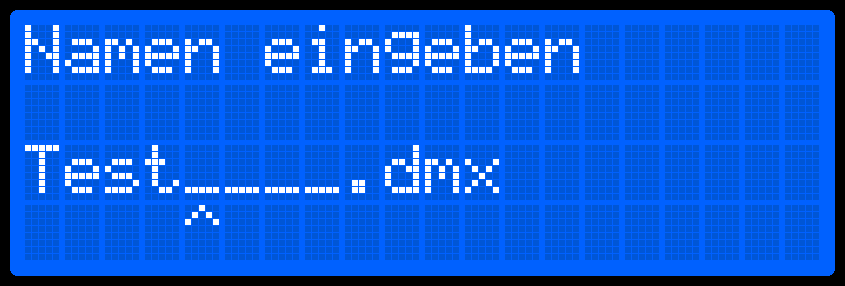
\includegraphics[width=.25\linewidth]{LCD-Screenshots/Namenauswahl}
		\caption{LCD-Ausgabe Dateinamen einstellen}
		\label{lcd:filename}
	\end{center}
\end{figure}
Umgesetzt wird dieser Programmteil mithilfe eines Zeichen-Arrays, dessen Anzahl an Zellen der Länge des Dateinamens entspricht. Die letzten vier Zellen des Arrays werden mit der Dateiendung ($.dmx$) beschrieben. Die Endung ist bei der Auswahl des Namens nicht veränderbar. Die restlichen Zellen des Arrays werden inital mit einem Unterstricht beschrieben und sollen damit dem Benutzer ein veränderbares Zeichen signalisieren. Ein Zeichen besteht aus einem Byte und kann somit 256 Werte annehmen, wobei jeder Wert einem Zeichen entspricht. Wird zum Beispiel der Wert der einem $a$ entspricht um 1 inkrementiert, so wird ein $b$ dargestellt. Aufgrund dieses Systems kann der Wert der Position des Encoder unmittelbar als Zeichen dargestellt werden und in die entsprechende Zelle des Arrays geschrieben werden. Eine Veränderung der Encoderposition bewirkt eine Änderung des gerade ausgewählten Zeichens.
% !TEX root = BA-Bauer.tex

\subsubsection{Aufnahme eines DMX-Datenpaketes}
Die Aufnahme eines DMX-Datenpaketes zählt zu den kritischsten Zeilen Programmcode dieser Arbeit. Wird das erste Datenbyte nicht registriert, hat das bei der Wiedergabe, aufgrund der seriellen Übertragung des DMX-Protokolls, Auswirkungen auf alle angeschlossenen Geräte. Das Prinzip der Aufnahme von DMX-Datenpaketen ist bereits in der Praxisprojektarbeit aufgezeigt und wird in dieser Arbeit optimiert.
Die Aufnahme eines Datenpaketes basiert auf den Interrupt-Events der UART-Schnittstelle. Bei jedem empfangenen oder gesendetem Datenbyte, erkannten Fehler der Übertragung oder der Schnittstelle wird ein globaler Interrupt ausgelöst. In der aufgerufenen Funktion wird identifiziert was den Interrupt ausgelöst hat und es wird ein entsprechender Code ausgeführt. Für die Aufnahme sind die Events des $Framing\ Errors$ und des erfolgreichen Empfangs eines Datenbytes von Bedeutung. Wie in der Praxisprojektarbeit wird mithilfe des $Framing\ Errors$ das Ende eines DMX-Datenpaketes erkannt. Codeausschnitt \ref{code:itSaveByte}, \ref{code:dmx.c-rxIT}, \ref{code:itFE}, \ref{code:itErrorclear} und \ref{code:itResetRx} zeigen Ausschnitte aus der globalen UART-Interruptfunktion, die wesentlich für den Empfang von DMX-Datenpaketen sind. Die folgende Funktion wird aufgerufen wenn ein Datenbyte ohne einen Fehler vollständig empfangen und bereit zum Lesen ist. 
\begin{lstlisting}[caption = stm32f4xx\_it.c: UART Save\_Byte\_Rx(),
label = code:itSaveByte, 
language = C, 
firstnumber = 442]
static void Save_Byte_Rx()
{
	*huart4.pRxBuffPtr++ = huart4.Instance->DR; //DR in Buffer speichern
	if(--huart4.RxXferCount == 0U)
	{
		//save to SD
		HAL_UART_RxCpltCallback(&huart4);
		Reset_Rx();
	}
}
\end{lstlisting}
Zunächst wird in Zeile 444 das eingegangene Datenbyte aus dem $DR$-Register der UART-Schnittstelle dem Zeiger auf das Puffer-Array (\textit{huart4.pRxBuffPtr}) zugewiesen und dieser anschließend um einer Stelle inkrementiert.
Darauf folgt eine $if$-Abfrage, die Identifiziert, ob alle erwarteten Datenbytes empfangen sind. Bei einem Aufruf der Empfangsfunktion $HAL\_UART\_Receive\_IT(...)$ zum Starten des Empfangsvorgangs der UART-Schnittstelle wird die Anzhal der zu empfangenen Datenbytes der Vaiable $RxXferCount$ zugewiesen und wird bei jedem empfangenen Datenbyte um eine Stelle dekrementiert. Enthält die Variable nach der Dekrementierung den Wert 0, so sind alle Datenbytes empfangen und ein entsprechender $Callback$ wird aufgerufen. Dieser befindet sich in der Datei $DMX.c$ und ist in Codeausschnitt \ref{code:rxIT} zu sehen. 
\lstinputlisting[
caption = DMX.c: Callback-Funktion eingehender UART-Daten,
label = code:dmx.c-rxIT, 
language = C, 
firstnumber = 103, 
firstline = 103, 
lastline = 113]
{/Users/Felix/Documents/CubeMX/BPA-Code/Core/Src/DMX.c}
Wenn die Callback Funktion aufgerufen wird, ist ein DMX-Datenpaket vollständig empfangen. Dem Hauptprogramm wird das mithilfe der Zuweisung der Variable $RxComplete$ mit dem Wert 1 signalisiert. Die Variable der Anzahl der empfangenen Datenpakete $received\_packets$ wird außerdem inkrementiert. Das Ein- bzw. Ausschalten der Empfangs-LED ($LED\_RX$) gibt dem Benutzer eine Rückmeldung über den erfolgreichen Empfang eines DMX-Datenpaketes. Ist durch das Hauptprogramm die Variable $recording$ nicht mit dem  Wert 1 beschrieben, also findet keine aktive Speicherung der Daten statt, wird die Status-LED ein- bzw. ausgeschaltet. Der Benutzer bekommt somit eine Rückmeldung über den Datenfluss bevor eine Aufnahme aktiv gestartet wird. Somit kann sichergagengen werden, dass DMX-Daten fehlerfrei eingehen und bei einem Start der Aufnahme keine unerwarteten Fehler im Bezug auf den Datenfluss auftreten.
\newline
Nach der Bearbeitung des Callbacks wird als letzter Schritt die Funktion $Reset\_Rx()$ (Codeausschnitt \,\ref{code:itResetRx})aufgerufen. In ihr werden alle Variablen der UART-Schnittstelle auf die für den Empfang eines neuen DMX-Datenpaketes benötigten Initialwerte zurückgesetzt.
\begin{lstlisting}[caption = stm32f4xx\_it.c: UART Reset\_Rx(),
	label = code:itResetRx, 
	language = C, 
	firstnumber = 434]
	static void Reset_Rx()	//Rx complete or Error ->dmx-brake
	{
		huart4.RxXferCount = 513;
		huart4.RxXferSize = 513;
		huart4.pRxBuffPtr = Univers.RxBuffer;
		(void)*huart4.pRxBuffPtr--;
	}
\end{lstlisting}
Das zweite wichtige Event der UART-Schnittstelle ist der $Framing-Error$ ($FE$) der das Ende des DMX-Datenpaketes signalisiert. Codausschnitt \ref{code:itFE} zeigt den Auschnitt der Behandlung eines $FE$ in der globalen Interrupt-Funktion der UART-Schnittstelle. Wird ein $FE$ identifiziert, so muss zunächst das Bit, welches den Error anzeigt zurückgesetzt werden damit die Funktion nicht unmittelbar nach dem Beenden ernuet aufgerufen wird.
\begin{lstlisting}[caption = stm32f4xx\_it.c: UART Framing Error,
	label = code:itFE, 
	language = C, 
	firstnumber = 349]
/* UART frame error interrupt occurred -----------------------------------*/
if (((isrflags & USART_SR_FE) != RESET) && ((cr3its & USART_CR3_EIE) != RESET))
{
	Clear_Rx_Error();
	huart4.ErrorCode |= HAL_UART_ERROR_FE;
}
\end{lstlisting}
Mithilfe der Funktion $Clear\_Rx\_Error()$, dessen Inhalt Codesausschnitt \ref{code:itErrorclear} zeigt, wird druch einen Lesevorgang des entsprechenden Status-Registers $SR$ und des Daten-Registers $DR$ alle gesetzten Bits auf den Initialwert zurückgesetzt. Anschließend wird die Funktion $Reset\_Rx()$ aufgerufen. Zuletzt wird der $ErrorCode$ der UART-Schnittstelle mit dem entsprechenden $FE$ Error-Code beschrieben. 
\begin{lstlisting}[caption = stm32f4xx\_it.c: UART Clear\_Rx\_Error(),
	label = code:itErrorclear, 
	language = C, 
	firstnumber = 426]
static void Clear_Rx_Error()
{
	uint16_t tmp = huart4.Instance->SR;
	tmp = huart4.Instance->DR;
	(void) tmp;
	Reset_Rx();
}
\end{lstlisting}
Dieser Ablauf findet außerdem bei allen anderen auftretenden Fehlern statt um fehlerhafte Datensätze zu verhindern. Nur wenn ein vollständiges Datenpaket empfangen ist oder das Datenpaket durch einen $FE$ als beendet erklärt ist, wird dieses für die Speicherung dem Hauptprogramm \"freigegeben\".\\
\newline
\textbf{Optimierungsmöglichkeiten}\\
Aus progammatischer Sicht ist die Verteilung des Codes über mehrere Dateien nicht besonders elegant und erschwert die Implementierung in zukünftigen Projekten. Besser wäre es den Code vollständig in den Dateien DMX.c und DMX.h unterzubringen. Das erleichtert die Übersichtlichkeit des Programms und beugt damit Fehlern vor. Zudem ist es sinnvoll jeden der bei der Übertragung auftretenden Fehler anders zu behandeln um z.B. eine Fehlerkorrektur durchzuführen und unnötig großen Datenverlust zu verhindern. Anstatt ein komplettes Datenpaket zu ignorieren sobald ein Byte fehlerhaft ist, könnte der Wert des Fehlerhaften Bytes aus dem vorherigen Datenpaket übernommen werden. Damit reduziert sich der Datenverlust von einem Datenpaket auf ein eventuell falsches Daten-Byte. Entsprechende Infomationen über den Anteil von Fehlerhaften Datenpaketen ober -Bytes könnten für den Benutzer ersichtlich dargestellt werden und eine Rückmeldung über die generelle Übetragungsqualität geben.
\subsubsection{Speicherung der Aufnahmedaten}
\label{sec:save_data}
Abbildung \ref{fig:DMXDatenformat} zeigt die Reihenfolge in der die einzelnen Bytes in der Aufnahme-Datei mit der Endung $.dmx$ gespeichert werden. Alle aufgenommenen Datenpakete werden hintereinander in der Datei gespeichert. Begonnen wird mit dem Zeitpunkt an dem das Datenpaket vollständig empfangen wurde. Alle vier Bytes der 32-Bit Variable werden hintereinander gespeichert. Darauf folgen die eigentlichen DMX-Informationen der einzelnen DMX-Kanäle. Auch diese werden nacheinander gespeichert, beginnend mit dem DMX-Startbyte (Kanal 0). Nach dem letzten Datenbyte des DMX-Datenpaketes befindet sich das Schlusszeichen (NPC) des Datenpaketes. Direkt nach dem Schlusszeichen beginnt das nächste Datenpaket. 
\begin{figure}[h]
	\begin{center}
		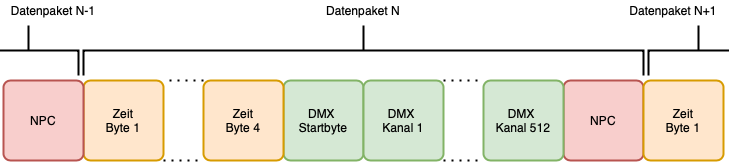
\includegraphics[width=\linewidth]{DMX-Datenformat}
		\caption{DMX-Aufnahmedaten Bytereihenfolge}
		\label{fig:DMXDatenformat}
	\end{center}
\end{figure} Geht man davon aus, dass die DMX-Datenpakete mit der maximal möglichen Frequenz von ca. 44,1\,Hz eingehen, so wird pro Minute ein Speicherplatz von:
\begin{equation}
	44,1\,Hz * 518\,Byte * 60\,s = 1370628\,Byte = 1,37\,MByte
\end{equation} auf der SD-Karte benötigt. Eine SD-Karte mit einer Kapazität von 32\,GByte bietet somit Speicherplatz für ca. 23346 Minuten aufnahme. Das entspricht einer Aufnahmedauer von etwas über 16\,Tagen. Begrenzender Faktor der maximalen Dauer einer Aufnahme stellt das $FAT$-Dateisystem dar. Es stellt nur 4-Bytes für die Angabe der Dateigröße zur Verfügung und begrenzt damit die maximale Dateigröße auf 4\,GB \cite[s. 128]{BetriebssystemeKompakt}. Eine Datei umfasst demnach maximal $2^{32}\,Byte$. Das entspricht einer maximalen kontinuierlichen Aufnahmedauer von:
\begin{equation}
	tAufnahme_{max} = \frac{2^{32}\,Byte}{518\,Byte * 44,1\,Hz * 60\,\frac{s}{min} * 60\,\frac{min}{h}} = 55,227\,h
\end{equation}
Diese Dauer sollte in den meisten Fällen ausreichend sein und könnte nur erweitert werden indem ein anderes Dateisystem verwendet wird, oder beim Erreichen der maximalen Dateigröße die Speicherung der Daten in einer zweiten Datei fortgeführt wird. 
Zusätzlich zu den DMX-Daten, werden generelle Informationen über die Aufnahme in einer separaten Datei mit der Endung $.nfo$ gespeichert. Alle Informationen werden unabhängig vom Aufnahmemodus gespeichert. Darunter befinden sich die Aufnahmedauer, die Anzahl der gespeicherten Datenpakete und das NPC-Byte.\\
\newline
\textbf{Optimierungsmöglichkeiten}\\
Die Datenpakete werden unabhängig vom Informationsgrad gespeichert, was unnötig viel Speicherplatz erfordert. Denkbar ist ein Vergleich des aktuell zu speichernden DMX-Datenpakets mit dem zuvor gespeicherten DMX-Datenpaket. Beinhaltet das zuvor gespeicherte DMX-Datenpaket die selben Informationen wie das aktuelle, so könnte die Speicherung des aktuellen Paketes übersprungen werden, da es keine neuen Informationen enthält. Dieser Vorgang benötigt allerdings Ressourcen um den Vergleich der Datenpakete vorzunehmen. Durch den Vergleich und das eventuelle wegfallen von Speicherungsvorgängen könnten widerrum Ressourcen eingespart werden.
% !TEX root = BA-Bauer.tex

\subsection{Wiedergabefunktion}
Für die Weidergabe der aufgenommenen DMX-Daten werden zwei Wiedergabemodi benötigt. Die Aufnahmedaten der Standard, Trigger und Endlosaufnahme werden für die Wiedergabe gleich behandelt. Die Aufnahmedaten der $Step$-Aufnahme widerrum müssen gesondert behandelt werden, da diese keine Zeitinformation enthalten. Für beide Aufnahmemodi muss zunächst die entsprechende Aufnahmedatei ausgewählt werden.

\subsubsection{Auswahl der Aufnahmedatei}
\label{sec:selectfile}
Um dem Benutzer eine Auswahl der Aufnahmedatei zu ermöglichen muss zunächst die SD-Karte nach vorhandenen Dateien durchsucht werden. Zudem müssen die Namen abgerufen und auf dem LCD-Display ausgegeben werden. Mithilfe der Funktion $f\_findfirst(..)$ kann die SD-Karte an einem bestimmten Dateipfad nach Dateien mit einem bestimmten Muster im Dateinamen durchsucht werden. Alle Aufnahmedateien werden mit der Endung $.dmx$ gespeichert. Das Suchmuster wird mit $*.dmx$ festgelegt und bedeutet, dass jede Datei dessen letzten vier Zeichen $.dmx$ beinhalten gefunden werden. Der Funkiont $f\_findfirst(...)$ wird zudem ein $FILINFO$ Struktur namens $info$ übergeben. Wird eine Datei passend zu dem festgelegten Suchmuster gefunden, so wird unter anderem der vollständige Dateiname in dem Zeichen-Array $info.fname$ gespeichert. Ist das Array leer, wurde keine Datei gefunden. Nachdem die erste Datei gefunden ist, müssen die restlichen auf der SD-Karte befindlichen Dateien gefunden werden. Dafür wird die Funktion $f_findnext(...)$ verwendet. Diese Funktion wird so lange aufgerufen, bis keine weitere Datei gefunden wird. Nach jedem erfolgreichen Aufruf wird der Dateiname in ein multidimensionales Zeichen-Array gespeichrt, welches 20 Dateinamen beinhalten kann. Der Inhalt dieses Arrays wird dazu benutzt die Dateinamen auf dem LCD-Display darzustellen. Durch drehen der Encoders wird die Auswahl verändert. Ist eine Auswahl getroffen wird sie mit dem Bestätigen-Taster bestätigt. Die Auswahl der Aufnahmedatei kann jederzeit durch betätigen des Zurück-Taster abgebrochen werden.\\
\newline
\textbf{Optimierungsmöglichkeiten}\\
Die Auswahlfunktion ist durch die Größe des multidimensionalen Zeichen-Arrays auf die Anzeige von maximal 20 Dateinamen begrenzt. Für die Weiterentwicklung der Software ist es sinnvoll eine Lösung zu finden bei der die Anzahl der maximal anzuzeigenden Dateien nicht begrenzt ist.

%Im Gegensatz zu den mehreren Aufnamefunktionen gibt es für die Wiedergabe der DMX-Daten nur eine Wiedergabefunktion. Aus den auf der SD-Karte während der Aufnahme gespeicherten Informationen in der $.nfo$-Datei kann bestimmt werden, wie die gespeicherten Daten wiedergegeben werden müssen. Zunächst startet die Funktion mit der Auswahl der wiederzugebenen Aufnahmedatei. Dafür wird die SD-Karte nach Dateien durchsucht die eine $.dmx$ Dateiendung besitzen. Die Dateinamen werden dann auf dem Display angezeigt und können durch das Drehen des Encoders ausgewählt werden. Mit dem Bestätigungs-Taster wird die Auswahl festgelegt und das erste Datenbyte gelesen. Auf dem Display erscheint eine Abfrage ob die Wiedergabe gestartet werden soll. Wird ein weiteres Mal der Bestätigungstaster betätigt, startet die Wiedergabe. Sie kann mit einer Betätigung des Zurück-Tasters gestoppt werden.

\subsubsection{Wiedergabe einer kontinuierlichen Aufnahme}
Nachdem eine Aufnahmedatei erfolgreich ausgewählt ist, wird die zugehörige Info-Datei geöffnet und die Daten gelesen. Ist die darin befindliche Aufnahmedauer größer als null, handelt es sich um eine kontinuierliche Aufnahme. Für die Wiedergabe der Standardmodus verwendet. Ein Flussdiagramm der Funktion befindet sich im Anhang \ref{fluss:playconti}. Als erstes wird ein Millisekunden Timer gestartet, woraufhin vier Bytes aus der Aufnahmedatei gelesen werden. Der Inhalt der ersten vier Bytes ist der bei der Aufnahme registrierte Zeitpunkt an dem das DMX-Datenpaket vollständig empfangen ist, wie in Kapitel \ref{sec:save_data} erläutert ist. Bei der Wiedergabe fungiert diese Zeit als Startzeitpunkt des jeweiligen Datenpaketes. Anschließend werden einzelne Bytes aus der Datei gelesen, bis entweder das Ende der Datei erreicht, die maximale Anzahl DMX-Kanälen eines Datenpaketes erreicht ist oder das NPC-Zeichen erkannt wird. Ist das Ende der Datei erreicht wird mithilfe der Funktion $f\_lseek(...)$ zum Beginn der Datei zurückgekehrt und der Zähler des gestarteten Timers auf 0 zurückgesetzt. Ist das NPC-Zeichen erkannt oder die maximale Anzahl an Bytes empfangen, so wird die am Anfang gelesene Startzeit des Datenpaketes mit dem Zähler des Timers verglichen, bis der Zähler den gleichen oder einen höheren Wert als die Startzeit besitzt. Erst danach wird das DMX-Datenpaket gesendet und die Funktion startet erneut mit dem Lesen der Startzeit des nächsten Datenpaketes. Die Wiedergabe kann durch die Betätigung des Zurück-Tasters beendet werden. Die Abfrage der Betätigung erfolgt jeweils vor dem Lesen der Startzeit.
% !TEX root = BA-Bauer.tex
\subsection{Ausgabe eines DMX-Datenpaketes}
Die Funktion zum Senden von DMX-Datenpakten wurde im Vergleich zu der Praxisarbeit optimiert und vereinfacht. Der Vollständige Sendevorgang wird mit nur zwei Funktionen ausgeführt. Codeausschnitt \ref{code:dmx.c-Transmit} zeigt die Funktion zum Senden eines DMX-Datenpaketes, welche als einzige aufgerufen werden muss um ein Datenpaket zu senden.
\lstinputlisting[
caption = DMX.c: Transmit-Funktion,
label = code:dmx.c-Transmit, 
language = C, 
firstnumber = 66, 
firstline = 66, 
lastline = 79]
{/Users/Felix/Documents/CubeMX/BPA-Code/Core/Src/DMX.c}
Die Übergabeparameter der Funktion sind eine DMX-Struktur ($struct$\footnote{text}) $DMX_TypeDef*\ hdmx$ und die Anzahl der zu übertragenden Datenbytes \textit{uint16\_t size}. In der DMX-Struktur befinden sich Informationen über die zu verwendende UART-Schnittstelle, %Macht nur Sinn wenn das im Code auch benutzt wird
sowie das Array $TxBuffer$ mit den zu übertragenen Datenbytes. Zu beginn der Funktion wird in Zeile 68 der Treiberchip über das Beschreiben des Pins $DMX\_DE\_Pin$ mit einem High-Pegel aktiviert. Daraufhin wird der Ausgangspin der UART-Schnittstelle mithilfe der Funktion $DMX\_set\_TX\_Pin\_manual()$ manuell beschreibbar gemacht und mit einem High-Pegel beschrieben. Das Prinzip dieses Vorgang ist in der Praxisarbeit beschrieben \cite{Bauer2021}. %Seite einfügen
Das Zählerregister ($CNT$) des Timers 11 (\textit{htim11}) wird mit dem Wert 0 überschrieben und das $UIF$-Bit \textit{Update Interrupt Flag} im Statusregister des Timers zurückgesetzt. Dieses Bit wird hardwareseitig gesetzt wenn der Timer übergelaufen ist. Mit der Funktion $SET\_BIT(...)$ wird das $CEN$ Bit gesetzt, wodurch der Timer startet. Der Timer ist zuvor in CubeMX als $one-pulse$-Timer%stimmt das??
konfiguriert. Sobald der Timer übergelaufen ist, wird er gestoppt und zählt den Zähler $CNT$ nicht weiter hoch. Mit der $while$-Abfrage in Zeile 74 wird auf den Überluf des Timers gewartet. Ist er übergelaufen, so wird das $UIF$-Bit wieder zurückgesetzt und der Ausgangspin in Zeile 76 mit einem Low-Pegel beschrieben. Zu diesem Zeitpunkt ist das DMX-Startsignal vollständig ausgegeben und die Datenbytes können gesendet werden. Um der UART-Schnittstelle wieder Zugriff auf den Ausgangspin zu gewähren wird mit der Funktion \textit{DMX\_set\_TX\_Pin\_auto()} die manuelle Beschreibbarkeit des Pins deaktiviert. Anschließend wird mit dem Funktionsaufruf in Zeile 78 die Übertragung der Daten gestartet. Bei dieser Funktion handelt es sich um eine nicht-blockierende Funktion. Die Daten werden Interruptbasiert gesendet. Sind alle Daten vollständig gesendet, so wird durch einen Interrupt der UART-Schnittstelle die Funktion in Codeausschnitt \ref{code:dmx.c-txIT} aufgerufen.
\lstinputlisting[
caption = DMX.c: Interrupt-Funktion ausgehender UART-Daten,
label = code:dmx.c-txIT, 
language = C, 
firstnumber = 120, 
firstline = 120, 
lastline = 128]
{/Users/Felix/Documents/CubeMX/BPA-Code/Core/Src/DMX.c}
Der Inhalt der Funktion soll nur ausgeführt werden, wenn ein aktiver Sendevorgang ausgeführt wird, also wenn die Variable \textit{Univers.sending} den Wert 1 enthält. Ist dies der Fall, so wird der UART-Ausgangspin ein weiteres Mal mit der Funktion \textit{DMX\_set\_DMX\_Pin\_manual} manuell beschreibbar gemacht und der Pin mit einem Low-Pegel beschrieben um das $Brake$-Signal des DMX-Protokolls zu senden. Anschließend wird der Zustand der entsprechenden LED invertiert um den Benutzer eine Rückmeldung über einen erfolgreichen Sendevorgang eines Datenpaketes zu geben.\\
\textbf{Optimierungsmöglichkeiten}\\
Wie auch in der Praxisarbeit wird das Signal ohne $Interbytedelay$, also Verzögerung zwischen den einzelnen Datenbytes, gesendet. Dadurch wird das eingehende SIgnal nicht originalgetreu wiedergegeben, jedoch antsteht daraus kein Datenverlust oder eine Veränderung der Wiedergabefrequenz der einzelnen Datenpakete. Außerdem wird in der aktuellen Version des Programmcodes das $Interbytedelay$ während der Aufnahme nicht gemessen oder registriert. Um diese Funktionalität bei der Wiedergabe zu implementieren muss zunächst eine entsprechende Messung des $Interbytedelays$ während der Aufnahme erfolgen.
% !TEX root = BA-Bauer.tex
\subsection{LCD}
Für die Programmierung des LCD-Displays wird ein HAL-Treiber (HD44780-Stm32HAL) von Olivier Van den Eede verwendet und erweitert. Die Treiberdateien befinden sich im Anhang \ref{CD-Anhang}. Der Treiber ist für die Steuerung von HD44780-Punktmatrixtreibern für LCD-Displays und ursprünglich für die Verwendung mit den Mikrokontrollern der STM32 F1-Serie entwickelt. Auf dem in dieser Arbeit verwendeten LCD-Modul befindet sich ein SPLC780-Treiberchip zum steuern des Displays und ist kompatibel mit den Anweisungen für HD44780-Treiberchips. Der Treiber kann LCD-Displays der Größe 16xN und 20xN Zeichen steuern. Standardmäßig ist die Größe 16x2 aktiviert, kann jedoch durch auskommentieren der entsprechenden Konstanten-Definition verändert werden. 
\begin{lstlisting}[firstnumber=16, language=C, caption = lcd.h: Einstellung Displaygröße, label = code:lcdsize]
	#define LCD20xN 		// For 20xN LCDs
	//#define LCD16xN			// For 16xN LCDs
\end{lstlisting}
Damit der Treiber mit den Mikrokontrollern der STM32 F4-Serie kompatibel ist, muss zudem die includierte Datei $stm32f1xx\_hal.h$ mit $stm32f4xx\_hal.h$ in der Header-Datei ersetzt werden.
\newline
Um das LCD-Display verwenden zu können benötigt der Treiber Informationen über die Verbindungen der Pins des LCD-Moduls mit den Pins des MCUs. Die Verbindungsinformationen werden für die Datenleitungen $D0$ bis $D7$ in zwei Arrays ($ports$ und $pins$), jeweils eins für Pin und Port, global gespeichert. Der Zellenindex (0-7) der Arrays entspricht der jeweiligen Datenleitung ($D0$-$D7$). Zusätzlich zu den Informationen zu den Datenleitungen werden die Informationen für den $RS$ und $EN$-Pin benötigt. Diese werden zusammen mit den Zeigern auf die Arrays $pins$ und $ports$ der Funktion $lcd\_create(...)$ (Codeausschnitt \ref{code:lcdcreate}) übergeben. Außerdem wird der 8-Bit Modus des Treibers durch die Übergabe des Prameters $LCD\_8\_BIT\_MODE$ aktiviert um schnellere Schreibraten zu erreichen, wie bereits in Kapitel \ref{sec:HardLCD} erläutert.
\begin{lstlisting}[firstnumber=302, language=C, caption = main.c: Funktionsaufruf lcd\_create(...), label = code:lcdcreate, breaklines = true]
lcd = Lcd_create(ports, pins, LCD_RS_GPIO_Port, LCD_RS_Pin, LCD_E_GPIO_Port, LCD_E_Pin, LCD_8_BIT_MODE);
\end{lstlisting}

Soll ein Zeichen an einer bestimmten Stelle des LCD-Displays gezeigt werden, so muss zunächst der sogenannte $cursor$ an der entsprechenden Stelle platziert werden. Für diesen Zweck ist die Funktion \textit{Lcd\_cursor(Lcd\_HandeTypeDef $*$ lcd, uint8\_t row, uint8\_t col)} im Treiber zu finden. Mit dem Parameter $row$ wird die Zeile und mit dem Parameter $col$ die Spalte der Position des Cursors festgelegt, wobei der Wert 0 der ersten Zeile oder Spalte entspricht. Der Cursor verschiebt sich um eine Stelle nach rechts nachdem ein neues Zeichen dargestellt ist. Ist das Ende einer Zeile erreicht, wird der Cursor an den Anfang der nächsten Zeile verschoben. Diese Funktionsweise ermöglicht es einzelne bereits dargestelle Zeichen zu überschreiben, ohne den Inhalt des gesamten LCD-Displays erneut beschreiben zu müssen.
\newline
Bei dem Beschreiben des Display sind des öfteren Fehler aufgetreten, bei dem zusätzliche, willkürliche Zeichen nach dem Ende der auszugebenden Zeichenkette ausgegeben werden. Der Grund für diesen Fehler ist die Unfähigkeit der Ausgabefunktion das Ende der Zeichenkette zu erkennen. Aus diesem Grund wird für die Ausgabe die zusätzliche Funktion $void\ Lcd\_string\_length(...)$ in Codeausschnitt \ref{code:stringlength} dem Treiber hinzugefügt, bei dessen Aufruf die Anzahl der auszugebenden Zeichen als Parameter übergeben wird. Damit kann sichergegangen werden, dass nur eine bestimmte Anzahl an Zeichen ausgegeben werden.
\begin{lstlisting}[firstnumber=95, language=C, caption = lcd.c: Funktion Lcd\_string\_length(...), label = code:stringlength]
void Lcd_string_length(Lcd_HandleTypeDef * lcd, char * string, uint8_t length)
{
	for(uint8_t i = 0; i < length; i++)
	{
		lcd_write_data(lcd, string[i]);
	}
}
\end{lstlisting}
Umgesetzt wird diese Funktion mit einer einfachen $for$-Schleife, dessen Anzahl an Wiederholungen durch den Übergabeparameter $uint8\_t\ length$ bestimmt werden. Mithilfe der Funktion $lcd\_write\_data(..)$ werden einzelne Bytes in das Datenregister des SPLC780-Chips geschrieben und auf dem LCD-Display ausgegeben.
Zum Treiber ist außerdem eine Funktion hinzugekommen, mit der eine gesamte Zeile des LCD-Displays zurückgesetzt werden kann. Die enstrpechende Zeile wird der Funktion übergeben und mithilfe einer $for$-Schleife jedes Zeichen der Zeile mit einem Leerzeichen überschrieben.\\
\newline
\textbf{Optimierungsmöglichkeiten}\\
Grundsätzlich bietet der Treiber eine stabile Grundlage für einfache Ausgaben auf dem Zeichen-LCD-Display, jedoch nur wenn die Funktion $lcd\_string\_length(...)$ mit der entsprechenden Anzahl an Zeichen der auszugebenden Zeichenkette aufgerufen wird. Dafür muss während der Programmierung die Anzahl der Zeichen in der Zeichenkette händisch bestimmt und der Funktion übergeben werden und bietet damit ein großes Fehlerpotential. Besser wäre eine zuverlässige und automatische Erkennung der Zeichenkettenlänge in der Funktion $lcd\_string(...)$.
% !TEX root = BA-Bauer.tex

\subsection{SD-Karte (SDIO)}

Die von CubeMX generierte Initialisierungs-Funktion der SDIO-Schnittstelle führt beim Start des Gerätes oft zu Fehlern, wodurch die SD-Karte weder gelesen noch beschrieben werden kann. In der Regel fällt das Programm dann in eine endlose Fehler-Funktion und ein Neustart des Geräts erwirkt keine Änderung. Um dieses Problem zu lösen, wird nach den von CubeMX generierten Initialisierungsfunktionen im Hauptprogramm eine weitere Funktion zur Initialisierung der Verbindung mit der SD-Karte aufgerufen, dessen wesentlicher Inhalt in Codeausschnitt \ref{code:SDinit} zu sehen ist.
\lstinputlisting[
caption = SD Initialisierungs-Funktion,
label = code:SDinit,
firstline = 284,
firstnumber = 284,
lastline = 295]
{/Users/Felix/Documents/CubeMX/BPA-Code/Core/Src/main.c}
Um eine SD-Karte verwenden zu können, muss diese als erstes mithilfe der Funktion $f\_mount(...)$ \"montiert\" werden. Dabei wird ein Dateisystem $filesystem$ und ein Dateipfad $path$ mit der Hardware verknüpft. Bei diesem Schritt treten in der Regel Fehler auf. Ist der Rückgabewert der Funktion $f\_mount(...)$ nicht $FR\_OK$ werden die Zeilen 285 bis 294 so lange wiederholt bis die SD-Karte erfolgreich montiert ist, denn ohne ein das Speichermedium ist das Gerät in einerlei Hinsicht benutzbar. Der aktuelle Status der SD-Karte wird als erstes der Variable $sd\_state$ zugewiesen. Befindet sich keine SD-Karte im SD-Kartenslot ($STA\_NODISK$) wird eine entsprechende Meldung über das LCD-Display an den Benutzer gegeben. Ist der Status der SD-Karte $STA\_NOINIT$, sow wird das Montieren de SD-Karte zunächst rückgängig gemacht, indem erneut die Funktion $f\_mount(...)$ aufgerufen wird, jedoch wird der Wert 0 als Dateisystem-Übergabeparameter der Funktion übergeben. daaufhin wird die Variable des Dateisystem mithilfe der $memset(...)$ Funktion mit 0 initiaisiert und eine erneute SD-Initialisierung gestartet. %Warum genau wird SD_initialize ausgeführt? path wird nicht zurückgesetzt?! Vielleicht um path zurückzusetzen?
Die Schleife startet erneut mit einem weiteren Versuch der Montierung.

Codeausschnitt \ref{code:SDread} zeigt einen Beispielhaften Ablauf eines Lesevorgangs von der SD-Karte. Der Vogang startet mit dem Öffnen einer Datei, zu sehen in Zeile 1009. Mit dem Parameter $FA\_READ$ wird der Funktion mitgeteilt, dass die Datei gelesen werden soll. Der Parameter $FA\_OPEN\_ALWAYS$ sorgt dafür, dass die Datei geöffnet wird wenn sie existiert, ansonsten wird eine Datei mit dem entspechenden Dateinamen erstellt. In dem gezeigten Beispiel wird von der Existenz der Datei ausgegangen. Mit dem Parameter $FA\_OPEN\_EXISTING$ wird eine bereits existierende Datei geöffnet. Falls sie nicht existiert gitb die Funktion einen entsprechenden Fehlercode zurück. Soll eine Datei beschrieben werden, muss der Parameter $FA\_WRITE$ übergeben werden.
\lstinputlisting[
caption = Beispiel Lesevorgang der SD-karte,
label = code:SDread,
firstline = 1009,
firstnumber = 1009,
lastline = 1016]
{/Users/Felix/Documents/CubeMX/BPA-Code/Core/Src/DMX.c}
Nachdem die Datei geöffnet ist, werden Daten mit der Funktion $f\_read(...)$ aus der Datei gelesen. Der erste Übergabeparameter ist das Objekt der Datei aus der gelesen werden soll. Darauf folgt die Adresse der Zielvariable in der die gelesen Daten gespeichert werden sollen. An dritter Stelle steht die Anzahl der zu lesenden Bytes. Der letzte Übergabeparameter ist die Adresse einer Variable in der die Anzahl der tatsächlich gelesenen Bytes gespeichert wird. Durch einen nachfolgenden Vergleich der Soll und Ist Anzahl der Bytes können Fehler identifiziert werden \cite{FATFS}. Nachdem alle Lesevorgänge beendet sind, muss die Datei mit der Funktion $f\_close(...)$ wieder gechlossen werden, da die Anzahl der gleichzeitig geöffneten Dateien begrenzt ist um Speicherprobleme auszuschließen.\\
\textbf{Optimierungsmöglichkeiten}\\
In der aktuellen Version des Programms wird der 1-Bit-Modus der SDIO-Schnittstelle verwendet. Von den vier vorhandenen Datenleitungen wird nur eine in diesem Modus verwendet. Auf der Platine sind zusätzliche Leiterbahnen für die Verwendung eines 4-Bit-Modus vorhanden. Scheinbar befinden sich Fehler in der SDIO-Bibliothek in CubeMX, wodurch der montier-Vorgang nicht durchgeführt werden kann. Durch die Verwendung des 4-Bit-Modus könnte die Lese- und Schreibgeschwindigkeit der SD-Karte im bestmöglichen Fall vervierfacht werden und trägt damit zur Stabilität während der Aufnahme und Wiedergabe bei.
% !TEX root = BA-Bauer.tex
\subsection{Menü}
Die Menüführung ist ein essentieller Bestandteil für die intuitive Bedienbarkeit des Gerätes. Sie muss leicht für den Benutzer zu durchschauen sein und mit den begrenzten Möglichkeiten der C-Programmiersprache programmierbar sein. Für die Menüführung wird ein einfaches Modell aus mehreren Ebenen verwendet. Nachdem das Gerät gestartet und alle Schnittstellen initialisiert sind, wird das Hauptmenü auf dem LCD angezeigt. Der Inhalt des Displays ist in Abbildung \ref{fig:lcdmain} zu sehen. Das Hauptmenü stellt Ebene 0, also die unterste Ebene des Menüs, dar. Zu Beginn ist der erste Menüeintrag gewählt und wird mit einem Pfeil in der ersten Spalte des LCD-Displays markiert. Durch drehen des Encoders kann der Pfeil und damit der ausgewählte Eintrag verändert werden. Eine Drehung im Uhrzeigersinn verschiebt die Auswahl nach unten, eine Drehung gegen den Uhrzeigersinn nach oben. Ist die auszuführende Funktion mithilfe des Pfeils ausgewählt, so kann mit der Betätigung des Bestätigungs-Tasters die nächste Ebene des Menüs erreicht werden. Mithilfe des Zurück-Tasters kann zu der vorherigen Ebene zurückgekehrt werden. Je nach Auswahl werden die Inhalte aus Abbildung \ref{fig:lcdplay}, \ref{fig:lcdrec} oder \ref{fig:lcdset} angezeigt. Da auf dem LCD lediglich vier Zeilen zu Anzeige zur Verfügung stehen, sind Abbildung \ref{fig:lcdrec} und \ref{fig:lcdset} um die nicht sichtbaren Zeilen gestreckt. 
\begin{figure}[h]
	\begin{minipage}{.22\linewidth}
		\centering
		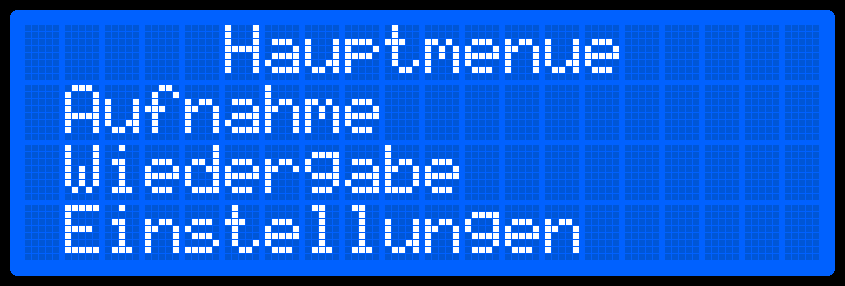
\includegraphics[width = \linewidth]{LCD-Screenshots/Hauptmenue}
		\caption{LCD-Hauptmenü}
		\label{fig:lcdmain}
	\end{minipage}
	\hfill
	\begin{minipage}{.22\linewidth}
		\centering
		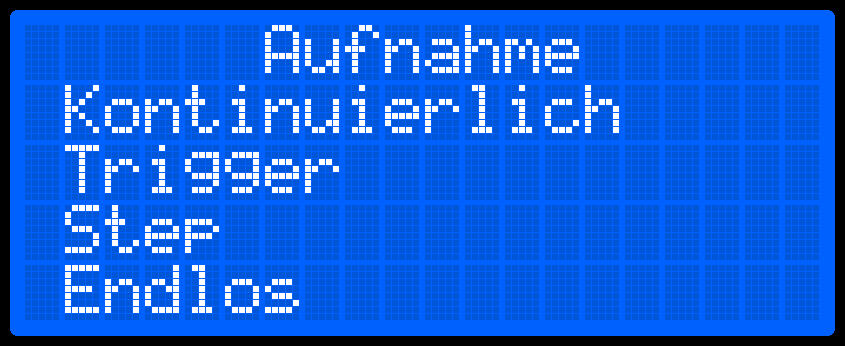
\includegraphics[width = \linewidth]{LCD-Screenshots/Aufnahme}
		\caption{LCD-Aufnahme}
		\label{fig:lcdrec}
	\end{minipage}
	\hfill
	\begin{minipage}{.22\linewidth}
		\centering
		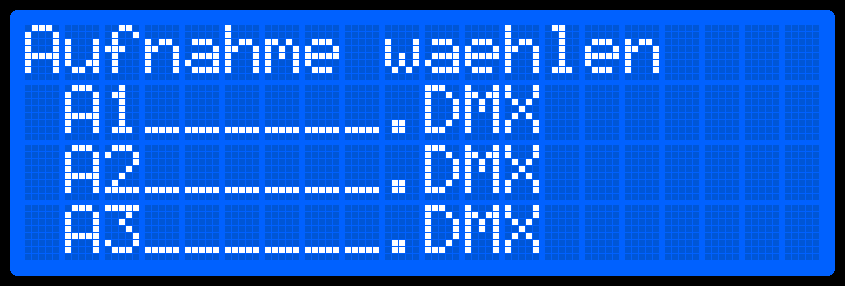
\includegraphics[width = \linewidth]{LCD-Screenshots/Wiedergabe}
		\caption{LCD-Wiedergabe}
		\label{fig:lcdplay}
	\end{minipage}
	\hfill
	\begin{minipage}{.22\linewidth}
		\centering
		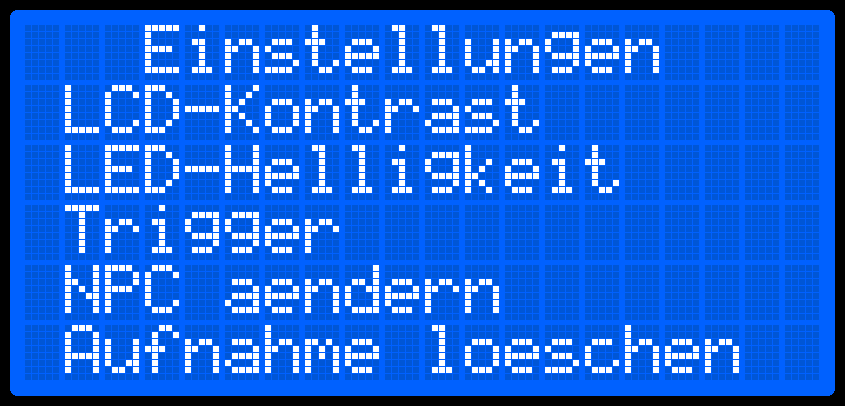
\includegraphics[width = \linewidth]{LCD-Screenshots/Einstellungen}
		\caption{LCD-Einstellungen}
		\label{fig:lcdset}
	\end{minipage}
\end{figure}
In Ebene 3 des Menüs befinden sich die tatsächlichen Funktionen zur Aufnahme und Wiedergabe der DMX-Daten und den Einstellungen. Im Hauptprogramm wird lediglich die Funktion $main\_menu(...)$ aufgerufen, um das Hauptmenü anzuzeigen. Die Zeichenketten, welche über das LCD-Display ausgegeben werden, sind in mehrdimensionalen $char$-Arrays definiert (Codeausschnitt \ref{code:menuarray}). Die erste Dimension des Arrays entspricht der Anzahl der anzuzeigenden Menüelemente, die zweite der Anzahl der zu beschreibenden Spalten des LCD-Displays. Es werden bewusst nur 19 Spalten der verfügbaren 20 mit den Menüelementen beschrieben, da vor jedem Element Platz für den Pfeil freigehalten wird, der die aktuelle Auswahl anzeigt. Um willkürliche Zeichen zu eliminieren, die sich eventuell noch in den nicht beschriebenen Speicherzellen der Arrays befinden, werden die nicht benötigten Zeichen mit Leerzeichen überschrieben.
\lstinputlisting[firstline = 13, firstnumber = 13, lastline = 18, language = C, caption =menu.c: Definition Zeichenkettenarray für LCD-Display-Ausgaben, label = code:menuarray]{/Users/Felix/Documents/CubeMX/BPA-Code/Core/Src/menu.c}
Durch die Verwendung der Zeichenkettenarrays können die Menüeinträge einfach verändert oder erweitert werden. Abbildung \ref{fig:flusshauptmenu} zeigt den Ablauf der Funktion $main\_menu(...)$. Zunächst werden alle Inhalte vom Display entfernt und die Menüüberschrift ausgegeben. Die globale Variable der Position des Encoders wird auf den Initialwert 0 zurückgesetzt. Daraufhin werden die ersten drei Menüeinträge aus dem Zeichenkettenarray unterhalb der Menüüberschrift ausgegeben (Abbildung \ref{fig:lcdmain}). Der Wert der Encoderposition entspricht der aktuellen Auswahl des Benutzers. Initial gilt der erste Eintrag als ausgewählt. Um nicht bei jedem Durchlauf der Funktion den gesamten Displayinhalt erneut ausgeben zu müssen erfolgt eine Abfrage ob sich die Encoderposition geändert hat. Nur wenn er sich verändert hat, wird der Auswahlpfeil an der entsprechend resultierenden Stelle angezeigt. Ist der Enter-Taster betätigt, wird die nächste entsprechende Menüebene aufgerufen.
\begin{figure}[h]
	\centering
	\includegraphics[width = .4\linewidth]{menue}
	\caption{Flussdiagramm Hauptmenü}
	\label{fig:flusshauptmenu}
\end{figure}
Welche Menüfunktion aufgerufen wird, wird mithilfe einer $switch-case$-Anweisung der Encoderposition entschieden. 
\newline
Um zu einer vorherigen Menüebene zurückzukehren, müssen die Menüfunktionen durch einen $return$-Befehl oder durch Erreichen des Endes der Funktion beendet werden. Werden die vorherigen Menüebenen in der jeweiligen Funktion durch einen Funktionsaufruf aufgerufen, kommt es zu einem rekursiven Aufruf von Funktionen. Zwangsläufig entstehen daraus Speicherprobleme, da reservierter Speicherplatz durch den Aufruf der Funktionen nicht wieder freigegeben wird. Ist der Speicher voll, so kommt es bei einem nächsten Funktionsaufruf zum Überlauf des Speichers und dadurch zu Fehlfunktionen oder vollständigem Abbruch des Programms.
% !TEX root = BA-Bauer.tex
\subsection{Einstellungen}
Dem Benutzer soll die Möglichkeit gegeben werden, bestimmte Anpassungen am Gerät vorzunehmen, um die Funktionsweise und Eigenschaften des Gerätes auf die eigenen Bedürfnisse anzupassen. In den folgenden Kapiteln wird auf die Einstellungsfunktionen eingegangen und deren Funktionsweise erläutert.
\subsubsection{LCD-Kontrast \& LED-Helligkeit}
Das Gerät kann durch die zahlreichen Einsatzgebiete auch an vielen verschiedenen Orten eingesetzt werden. Um zu garantieren, dass die auf dem LCD angezeigten Inhalte jederzeit erkennbar sind, soll der Benutzer die Möglichkeit haben den Kontrastwert des LCDs einzustellen. Gleiches gilt für die Helligkeit der LEDs. Soll das Gerät an einem unauffälligen Ort platziert werden, könnten aufblinkende LEDs stören. Aus diesem Grund sind die Einstellungsfunktionen zum Einstellen des LCD-Kontrastes und der LED-Helligkeit implementiert. In diesem Kapitel wird auf das Prinzip beider Funktionen eingegangen. Beide Einstellungen basieren auf dem gleichen Prinzip, der PWM-Steuerung. \\
\newline
\textbf{LCD-Kontrast}\\
In der Regel wird mithilfe eines einstellbaren Spannungsteilers (Potentiometer) eine Spannung an den $V0$-Pin des LCD-Moduls angelegt und damit der Kontrast geregelt. Diese verschiedenen Spannungswerte können auch mithilfe eines PWM-Signals erzeugt werden. Abbildung \ref{fig:lcdk25}, \ref{fig:lcdk50} und \ref{fig:lcdk75} zeigen die Auswirkungen der Änderung der Pulsweite auf den Kontrast des LCD-Displays. 
\begin{figure}[h]
	\begin{minipage}{.3\linewidth}
		\centering
		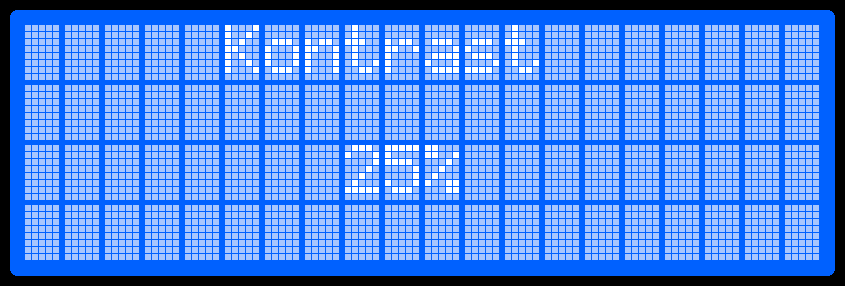
\includegraphics[width=\linewidth]{LCD-Screenshots/LCDKontrast25}
		\caption{LCD 25\% Kontrast}
		\label{fig:lcdk25}
	\end{minipage}
	\hfill
	\begin{minipage}{.3\linewidth}
		\centering
		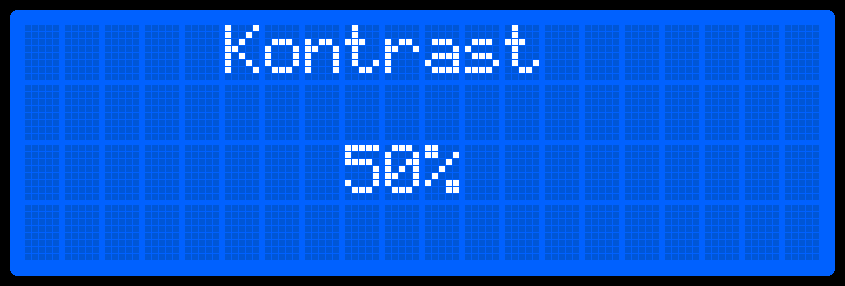
\includegraphics[width=\linewidth]{LCD-Screenshots/LCDKontrast50}
		\caption{LCD 50\% Kontrast}
		\label{fig:lcdk50}
	\end{minipage}
	\hfill
	\begin{minipage}{.3\linewidth}
		\centering
		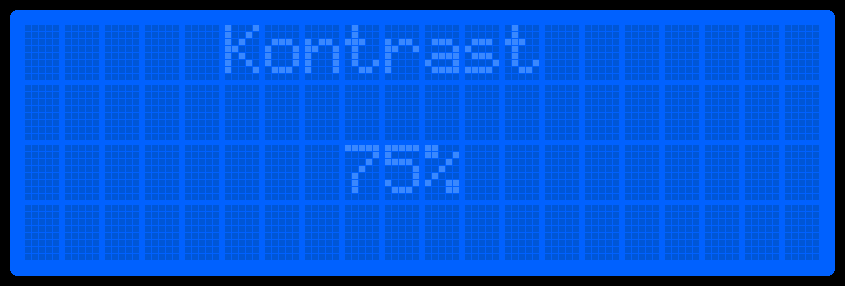
\includegraphics[width=\linewidth]{LCD-Screenshots/LCDKontrast75}
		\caption{LCD 75\% Kontrast}
		\label{fig:lcdk75}
	\end{minipage}
	\hfill
\end{figure}
Der Kontrastwert wird mithilfe des Encoders verändert und wird entsprechend auf dem Display angezeigt. Der Wert wird bei einer Drehbewegung im Uhrzeigersinn erhöht und bei einer Drehung gegen den Uhrzeigersinn verringert.\\
Für die Erzeugung des PWM-Signals wird Timer 1 des MCUs verwendet, welcher mit einer Frequenz von 10\,kHz Pulse an einem Ausgangspin erzeugt, der mit dem $V0$-Pin des LCD-Moduls verbunden ist. Die Pulsweite wird durch das Beschreiben des $CCR$-Registers\footnote{Capture Compare Register} mit Werten von 0-100 eingestellt. In der Einstellungsfunktion entspricht der Wert des $CCR$-Registers dem Kontrastwert in \%. Das Signal des Ausgangspins des Timer wird in Abbildung \ref{fig:PWM25} mit einer Pulsweite von 25\%, in Abbildung \ref{fig:PWM75} mit einer Pulsweite von 75\% gezeigt. 
\begin{figure}[h]
	\begin{minipage}{.48\linewidth}
		\centering
		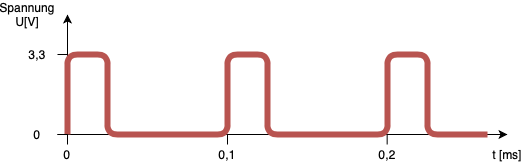
\includegraphics[width=\linewidth]{PWM25}
		\caption{10\,kHz PWM-Signal mit 25\% Pulsweite}
		\label{fig:PWM25}
	\end{minipage}
	\hfill
	\begin{minipage}{.48\linewidth}
		\centering
		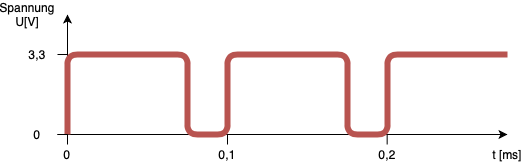
\includegraphics[width=\linewidth]{PWM75}
		\caption{10\,kHz PWM-Signal mit 75\% Pulsweite}
		\label{fig:PWM75}
	\end{minipage}
\end{figure}
\\
\newline
\textbf{LED-Helligkeit}\\
Wie auch der Kontrast des LCDs wird die Helligkeit der LEDs mithilfe eines PWM-Signals eingestellt. Für die LEDs wird Timer 9 des MCUs mit einer Pulsfrequenz von 12,5\,kHz verwendet. Bei dieser Frequenz ist bei niedrigen Helligkeiten kein Flackern der LEDs zu erkennen. Um den Effekt der Einstellung sichtbar zu machen, wird eine LED während der Einstellungsfunktion eingeschaltet. Die Einstellung der LED-Helligkeit unterscheidet sich von der Einstellung des LCD-Kontrasts lediglich in der auf dem LCD angezeigten Überschrift und durch die Verwendung eines anderen Timers und zu beschreibenden Registers.
\subsubsection{NPC ändern}
Das Zeichen, welches in der Aufnahmedatei zum Signalisieren des Datenpaketendes genutzt wird (NPC-Zeichen), ist initial 1. Die eingehenden DMX-Datenpakete werden während der Aufnahme nach diesem Zeichen durchsucht und durch ein anderes Zeichen (0) ersetzt. In speziellen Fällen wird das NPC-Zeichen explizit für die Steuerung von DMX-Geräten benötigt. Um eine Aufnahme der Daten und eine vollständig kompatible Wiedergabe der Daten trotzdem zu ermöglichen, hat der Benutzer die Möglichkeit das NPC-Zeichen und das entsprechende Ersatzzeichen frei zu wählen. 
\begin{figure}[h]
	\begin{center}
		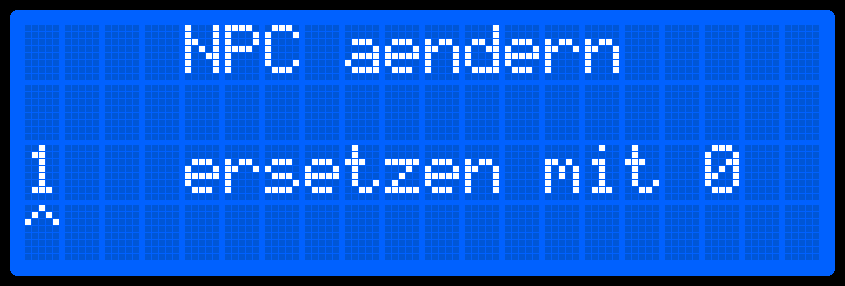
\includegraphics[width=.3\linewidth]{LCD-Screenshots/NPC}
		\caption{LCD-Ausgabe NPC Einstellung}
		\label{fig:npc}
	\end{center}
\end{figure}
Abbildung \ref{fig:npc} zeigt den Inhalt des LCDs der NPC-Einstellungsfunktion. Das Zeichen in der untersten Zeile des Displays signalisiert die aktuelle Auswahl und kann mit den Links- und Rechts-Tastern verändert werden. Der ausgewählte Wert wird mit der Drehung des Encoders eingestellt. Ist eine Auswahl getroffen, muss sie mit dem Bestätigen-Taster bestätigt werden. Daraufhin wird überprüft, ob beide Werte unterschiedlich sind. Sind beide Werte identisch, wird eine Fehlermeldung über den LCD ausgegeben. Andernfalls werden die Werte gespeichert und die Funktion kehrt zum Menü zurück. Die Funktion kann zudem jederzeit durch die Betätigung des Zurück-Tasters beendet werden.
\subsubsection{Trigger}
Um eine $Trigger$-Aufnahme zu starten muss ein $Trigger$-Wert eines bestimmten $Trigger$-DMX-Kanals überschritten werden, wie in Kapitel \ref{sec:recfunctions} erläutert ist. Um dem Benutzer auch hier die Möglichkeit einer Personalisierung zu geben, sind der $Trigger$-Kanal und -Wert vom Benutzer in den Einstellungen frei wählbar. Dadurch kann der Benutzer die Adressen der DMX-Geräte ohne Einschränkungen vergeben und anschließend einen entsprechenden freien Kanal für die $Trigger$-Funktionalität in den Einstellungen auswählen. 
\begin{figure}[h]
	\begin{center}
		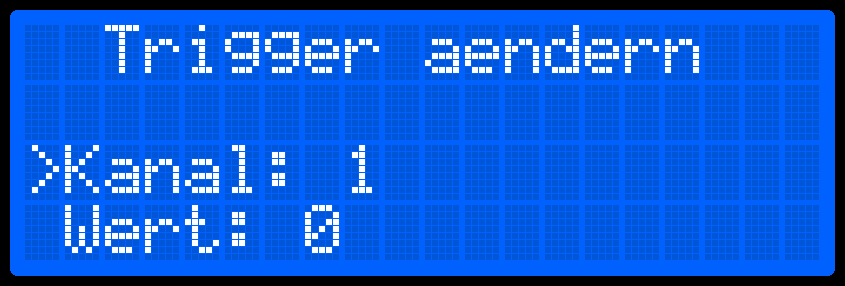
\includegraphics[width=.3\linewidth]{LCD-Screenshots/Trigger}
		\caption{LCD-Ausgabe Trigger-Einstellung}
		\label{fig:trig}
	\end{center}
\end{figure}
Abbildung \ref{fig:trig} zeigt die Ausgabe der Trigger-Einstellungsfunktion auf dem LCD. Ein Zeichen in der ersten Spalte des LCDs zeigt die aktuelle Auswahl an. Der Kanal bzw. der Wert wird durch Drehen des Encoders verändert. Es können Kanäle im Bereich von 0 bis 512 und Werte im Bereich von 1 bis 255 eingestellt werden. 
\subsubsection{Aufnahme löschen}
In dieser Einstellungsfunktion hat der Benutzer die Möglichkeit Aufnahmen zu löschen. Die Funktion durchsucht zunächst die SD-Karte nach Dateien mit der Endung $.dmx$ und zeigt deren Namen auf dem LCD an. Durch drehen des Encoders kann die zu löschende Datei ausgewählt werden, welche mit einem vor dem Dateinamen befindlichen Pfeil angezeigt wird. Für die Auswahl der Datei wird dieselbe Funktion verwendet, die in der Wiedergabefunktion Anwendung findet (Kapitel \ref{sec:selectfile}). Wird die Auswahl mit dem Bestätigen-Taster bestätigt, wird der Benutzer durch eine entsprechende Anzeige auf dem LCD zum Bestätigen des Löschvorgangs aufgefordert. Wird auch diese bestätigt, wird die entsprechende Aufnahme- und zugehörige Info-Datei gelöscht. Wird jedoch der Zurück-Taster betätigt, kehrt die Funktion zum Menü zurück. Der Löschvorgang wird mit der Funktion $f\_unlink()$ der FATFS-Bibliothek durchgeführt. Die Daten werden dabei nicht gelöscht, sondern lediglich die entsprechenden Speicherplätze wieder freigegeben, also aus der Dateizuordnungsliste des Dateisystems entfernt.